\chapter{Regular Expressions}\label{regexp}

\epigraphhead[30]{
\epigraph{\hspace*{-.1cm}\itshape``Some people, when confronted with a problem, think `I know, I'll use regular expressions.' Now they have two problems.''}%
{---Jamie Zawinski}
}\index{Zawinski, Jamie}\index{evolution}\index{adoption}\index{integration}

Programming \index{tool}tools and techniques survive and spread in a chaotic, evolutionary way. It's not always the pretty or brilliant ones that win but rather the ones that function well enough within the right niche or that happen to be integrated with another successful piece of technology.\index{domain-specific language}

In this chapter, I will discuss one such tool, \emph{\index{regular
expression}regular
expressions}. Regular expressions are a way to describe \index{pattern}patterns in string data. They form a small, separate language that is part of JavaScript and many other languages and systems.\index{interface!design}

Regular expressions are both terribly awkward and extremely useful. Their syntax is cryptic, and the programming interface JavaScript provides for them is clumsy. But they are a powerful \index{tool}tool for inspecting and processing strings. Properly understanding regular expressions will make you a more effective programmer.

\section{Creating a regular expression}\index{regular expression!creation}\index{RegExp class}\index{literal expression}\index{slash character}

A regular expression is a type of object. It can be either constructed with the \lstinline`RegExp` constructor or written as a literal value by enclosing a pattern in forward slash (\lstinline`/`) characters.

\begin{lstlisting}
let re1 = new RegExp("abc");
let re2 = /abc/;
\end{lstlisting}
\noindent

Both of those regular expression objects represent the same \index{pattern}pattern: an \emph{a} character followed by a \emph{b} followed by a \emph{c}.\index{backslash character!in regular expressions}\index{RegExp class}

When using the \lstinline`RegExp` constructor, the pattern is written as a normal string, so the usual rules apply for backslashes.\index{regular expression!escaping}\index{escaping!in regexps}\index{slash character}

The second notation, where the pattern appears between slash characters, treats backslashes somewhat differently. First, since a forward slash ends the pattern, we need to put a backslash before any forward slash that we want to be \emph{part} of the pattern. In addition, backslashes that aren't part of special character codes (like \lstinline`\n`) will be \emph{preserved}, rather than ignored as they are in strings, and change the meaning of the pattern. Some characters, such as question marks and plus signs, have special meanings in regular expressions and must be preceded by a backslash if they are meant to represent the character itself.

\begin{lstlisting}
let eighteenPlus = /eighteen\+/;
\end{lstlisting}
\noindent

\section{Testing for matches}\index{matching}\index{test method}\index{regular expression!methods}

Regular expression objects have a number of methods. The simplest one is \lstinline`test`. If you pass it a string, it will return a \index{Boolean}Boolean telling you whether the string contains a match of the pattern in the expression.

\begin{lstlisting}
console.log(/abc/.test("abcde"));
// → true
console.log(/abc/.test("abxde"));
// → false
\end{lstlisting}
\noindent\index{pattern}

A \index{regular expression}regular expression consisting of only nonspecial characters simply represents that sequence of characters. If \emph{abc} occurs anywhere in the string we are testing against (not just at the start), \lstinline`test` will return \lstinline`true`.

\section{Sets of characters}\index{regular expression}\index{indexOf method}

Finding out whether a string contains \emph{abc} could just as well be done with a call to \lstinline`indexOf`. Regular expressions allow us to express more complicated \index{pattern}patterns.

Say we want to match any \index{number}number. In a regular expression, putting a \index{set}set of characters between square brackets makes that part of the expression match any of the characters between the brackets.

Both of the following expressions match all strings that contain a \index{digit}digit:

\begin{lstlisting}
console.log(/[0123456789]/.test("in 1992"));
// → true
console.log(/[0-9]/.test("in 1992"));
// → true
\end{lstlisting}
\noindent\index{hyphen character}

Within square brackets, a hyphen (\lstinline`-`) between two characters can be used to indicate a \index{range}range of characters, where the ordering is determined by the character's \index{Unicode}Unicode number. Characters 0 to 9 sit right next to each other in this ordering (codes 48 to 57), so \lstinline`[0-9]` covers all of them and matches any \index{digit}digit.\index{whitespace!matching}\index{alphanumeric character}\index{period character}

A number of common character groups have their own built-in shortcuts. Digits are one of them: \lstinline`\d` means the same thing as \lstinline`[0-9]`.\index{newline character}\index{whitespace!matching}

\noindent\begin{tabular}{ll}
\lstinline`\d` &
Any \index{digit}digit character
\tabularnewline
\lstinline`\w` &
An alphanumeric character (``\index{word character}word character'')
\tabularnewline
\lstinline`\s` &
Any whitespace character (space, tab, newline, and similar)
\tabularnewline
\lstinline`\D` &
A character that is \emph{not} a digit
\tabularnewline
\lstinline`\W` &
A nonalphanumeric character
\tabularnewline
\lstinline`\S` &
A nonwhitespace character
\tabularnewline
\lstinline`.` &
Any character except for newline
\tabularnewline
\end{tabular}

So you could match a \index{date}date and \index{time}time format like 01-30-2003 15:20 with the following expression:

\begin{lstlisting}
let dateTime = /\d\d-\d\d-\d\d\d\d \d\d:\d\d/;
console.log(dateTime.test("01-30-2003 15:20"));
// → true
console.log(dateTime.test("30-jan-2003 15:20"));
// → false
\end{lstlisting}
\noindent\index{backslash character!in regular expressions}

That looks completely awful, doesn't it? Half of it is backslashes, producing a background noise that makes it hard to spot the actual \index{pattern}pattern expressed. We'll see a slightly improved version of this expression \hyperref[regexp.date_regexp_counted]{later}.\index{escaping!in regexps}\index{regular expression}\index{set}

These backslash codes can also be used inside \index{square brackets}square brackets. For example, \lstinline`[\d.]` means any digit or a period character. But the period itself, between square brackets, loses its special meaning. The same goes for other special characters, such as \lstinline`+`.\index{square brackets}\index{inversion}\index{caret character}

To \emph{invert} a set of characters—that is, to express that you want to match any character \emph{except} the ones in the set—you can write a caret (\lstinline`^`) character after the opening bracket.

\begin{lstlisting}
let notBinary = /[^01]/;
console.log(notBinary.test("1100100010100110"));
// → false
console.log(notBinary.test("1100100010200110"));
// → true
\end{lstlisting}
\noindent

\section{Repeating parts of a pattern}\index{regular expression!repetition}

We now know how to match a single digit. What if we want to match a whole number—a \index{sequence}sequence of one or more \index{digit}digits?\index{plus character}\index{repetition}\index{+ operator}

When you put a plus sign (\lstinline`+`) after something in a regular expression, it indicates that the element may be repeated more than once. Thus, \lstinline`/\d+/` matches one or more digit characters.

\begin{lstlisting}
console.log(/'\d+'/.test("'123'"));
// → true
console.log(/'\d+'/.test("''"));
// → false
console.log(/'\d*'/.test("'123'"));
// → true
console.log(/'\d*'/.test("''"));
// → true
\end{lstlisting}
\noindent\index{* operator}\index{asterisk}

The star (\lstinline`*`) has a similar meaning but also allows the pattern to match zero times. Something with a star after it never prevents a pattern from matching—it'll just match zero instances if it can't find any suitable text to match.\index{British English}\index{American English}\index{question mark}

A question mark makes a part of a pattern \emph{\index{optional}optional}, meaning it may occur zero times or one time. In the following example, the \emph{u} character is allowed to occur, but the pattern also matches when it is missing.

\begin{lstlisting}
let neighbor = /neighbou?r/;
console.log(neighbor.test("neighbour"));
// → true
console.log(neighbor.test("neighbor"));
// → true
\end{lstlisting}
\noindent\index{repetition}\index{braces!in regular expression}

To indicate that a pattern should occur a precise number of times, use braces. Putting \lstinline`{4}` after an element, for example, requires it to occur exactly four times. It is also possible to specify a \index{range}range this way: \lstinline`{2,4}` means the element must occur at least twice and at most four times.

\label{regexp.date_regexp_counted}Here is another version of the \index{date}date and \index{time}time pattern that allows both single- and double-\index{digit}digit days, months, and hours. It is also slightly easier to decipher.

\begin{lstlisting}
let dateTime = /\d{1,2}-\d{1,2}-\d{4} \d{1,2}:\d{2}/;
console.log(dateTime.test("1-30-2003 8:45"));
// → true
\end{lstlisting}
\noindent

You can also specify open-ended \index{range}ranges when using braces by omitting the number after the comma. So, \lstinline`{5,}` means five or more times.

\section{Grouping subexpressions}\index{regular expression!grouping}\index{grouping}\index{parentheses!in regular expressions}

To use an operator like \lstinline`*` or \lstinline`+` on more than one element at a time, you have to use parentheses. A part of a regular expression that is enclosed in parentheses counts as a single element as far as the operators following it are concerned.

\begin{lstlisting}
let cartoonCrying = /boo+(hoo+)+/i;
console.log(cartoonCrying.test("Boohoooohoohooo"));
// → true
\end{lstlisting}
\noindent\index{crying}

The first and second \lstinline`+` characters apply only to the second \emph{o} in \emph{boo} and \emph{hoo}, respectively. The third \lstinline`+` applies to the whole group \lstinline`(hoo+)`, matching one or more sequences like that.\index{case sensitivity}\index{capitalization}\index{regular expression!flags}

The \lstinline`i` at the end of the expression in the example makes this regular expression case insensitive, allowing it to match the uppercase \emph{B} in the input string, even though the pattern is itself all lowercase.

\section{Matches and groups}\index{regular expression!grouping}\index{exec method}\index{array!RegExp match}

The \lstinline`test` method is the absolute simplest way to match a regular expression. It tells you only whether it matched and nothing else. Regular expressions also have an \lstinline`exec` (execute) method that will return \lstinline`null` if no match was found and return an object with information about the match otherwise.

\begin{lstlisting}
let match = /\d+/.exec("one two 100");
console.log(match);
// → ["100"]
console.log(match.index);
// → 8
\end{lstlisting}
\noindent\index{index property}\index{string!indexing}

An object returned from \lstinline`exec` has an \lstinline`index` property that tells us \emph{where} in the string the successful match begins. Other than that, the object looks like (and in fact is) an array of strings, whose first element is the string that was matched. In the previous example, this is the sequence of \index{digit}digits that we were looking for.\index{string!methods}\index{match method}

String values have a \lstinline`match` method that behaves similarly.

\begin{lstlisting}
console.log("one two 100".match(/\d+/));
// → ["100"]
\end{lstlisting}
\noindent\index{grouping}\index{capture group}\index{exec method}

When the regular expression contains subexpressions grouped with parentheses, the text that matched those groups will also show up in the array. The whole match is always the first element. The next element is the part matched by the first group (the one whose opening parenthesis comes first in the expression), then the second group, and so on.

\begin{lstlisting}
let quotedText = /'([^']*)'/;
console.log(quotedText.exec("she said 'hello'"));
// → ["'hello'", "hello"]
\end{lstlisting}
\noindent\index{capture group}

When a group does not end up being matched at all (for example, when followed by a question mark), its position in the output array will hold \lstinline`undefined`. Similarly, when a group is matched multiple times, only the last match ends up in the array.

\begin{lstlisting}
console.log(/bad(ly)?/.exec("bad"));
// → ["bad", undefined]
console.log(/(\d)+/.exec("123"));
// → ["123", "3"]
\end{lstlisting}
\noindent\index{exec method}\index{regular expression!methods}\index{extraction}

Groups can be useful for extracting parts of a string. If we don't just want to verify whether a string contains a \index{date}date but also extract it and construct an object that represents it, we can wrap parentheses around the digit patterns and directly pick the date out of the result of \lstinline`exec`.

But first we'll take a brief detour, in which we discuss the built-in way to represent date and \index{time}time values in JavaScript.

\section{The Date class}\index{constructor}\index{Date class}

JavaScript has a standard class for representing \index{date}dates—or, rather, points in \index{time}time. It is called \lstinline`Date`. If you simply create a date object using \lstinline`new`, you get the current date and time.

\begin{lstlisting}
console.log(new Date());
// → Mon Nov 13 2017 16:19:11 GMT+0100 (CET)
\end{lstlisting}
\noindent\index{Date class}

You can also create an object for a specific time.

\begin{lstlisting}
console.log(new Date(2009, 11, 9));
// → Wed Dec 09 2009 00:00:00 GMT+0100 (CET)
console.log(new Date(2009, 11, 9, 12, 59, 59, 999));
// → Wed Dec 09 2009 12:59:59 GMT+0100 (CET)
\end{lstlisting}
\noindent\index{zero-based counting}\index{interface!design}

JavaScript uses a convention where month numbers start at zero (so December is 11), yet day numbers start at one. This is confusing and silly. Be careful.

The last four arguments (hours, minutes, seconds, and milliseconds) are optional and taken to be zero when not given.\index{getTime method}

Timestamps are stored as the number of milliseconds since the start of 1970, in the UTC \index{time zone}time zone. This follows a convention set by ``\index{Unix time}Unix time'', which was invented around that time. You can use negative numbers for times before 1970. The \lstinline`getTime` method on a date object returns this number. It is big, as you can imagine.

\begin{lstlisting}
console.log(new Date(2013, 11, 19).getTime());
// → 1387407600000
console.log(new Date(1387407600000));
// → Thu Dec 19 2013 00:00:00 GMT+0100 (CET)
\end{lstlisting}
\noindent\index{Date.now function}\index{Date class}

If you give the \lstinline`Date` constructor a single argument, that argument is treated as such a millisecond count. You can get the current millisecond count by creating a new \lstinline`Date` object and calling \lstinline`getTime` on it or by calling the \lstinline`Date.now` function.\index{getFullYear method}\index{getMonth method}\index{getDate method}\index{getHours method}\index{getMinutes method}\index{getSeconds method}\index{getYear method}

Date objects provide methods such as \lstinline`getFullYear`, \lstinline`getMonth`, \lstinline`getDate`, \lstinline`getHours`, \lstinline`getMinutes`, and \lstinline`getSeconds` to extract their components. Besides \lstinline`getFullYear` there's also \lstinline`getYear`, which gives you the year minus 1900 (\lstinline`98` or \lstinline`119`) and is mostly useless.\index{capture group}\index{getDate method}\index{parentheses!in regular expressions}

Putting parentheses around the parts of the expression that we are interested in, we can now create a date object from a string.

\begin{lstlisting}
function getDate(string) {
  let [_, month, day, year] =
    /(\d{1,2})-(\d{1,2})-(\d{4})/.exec(string);
  return new Date(year, month - 1, day);
}
console.log(getDate("1-30-2003"));
// → Thu Jan 30 2003 00:00:00 GMT+0100 (CET)
\end{lstlisting}
\noindent\index{destructuring}\index{underscore character}

The \lstinline`_` (underscore) binding is ignored and used only to skip the full match element in the array returned by \lstinline`exec`.

\section{Word and string boundaries}\index{matching}\index{regular expression!boundary}

Unfortunately, \lstinline`getDate` will also happily extract the nonsensical date 00-1-3000 from the string \lstinline`"100-1-30000"`. A match may happen anywhere in the string, so in this case, it'll just start at the second character and end at the second-to-last character.\index{boundary}\index{caret character}\index{dollar sign}

If we want to enforce that the match must span the whole string, we can add the markers \lstinline`^` and \lstinline`$`. The caret matches the start of the input string, whereas the dollar sign matches the end. So, \lstinline`/^\d+$/` matches a string consisting entirely of one or more digits, \lstinline`/^!/` matches any string that starts with an exclamation mark, and \lstinline`/x^/` does not match any string (there cannot be an \emph{x} before the start of the string).\index{word boundary}\index{word character}

If, on the other hand, we just want to make sure the date starts and ends on a word boundary, we can use the marker \lstinline`\b`. A word boundary can be the start or end of the string or any point in the string that has a word character (as in \lstinline`\w`) on one side and a nonword character on the other.

\begin{lstlisting}
console.log(/cat/.test("concatenate"));
// → true
console.log(/\bcat\b/.test("concatenate"));
// → false
\end{lstlisting}
\noindent\index{matching}

Note that a boundary marker doesn't match an actual character. It just enforces that the regular expression matches only when a certain condition holds at the place where it appears in the pattern.

\section{Choice patterns}\index{branching}\index{regular expression!alternatives}\index{farm example}

Say we want to know whether a piece of text contains not only a number but a number followed by one of the words \emph{pig}, \emph{cow}, or \emph{chicken}, or any of their plural forms.

We could write three regular expressions and test them in turn, but there is a nicer way. The \index{pipe character}pipe character (\lstinline`|`) denotes a \index{choice}choice between the pattern to its left and the pattern to its right. So I can say this:

\begin{lstlisting}
let animalCount = /\b\d+ (pig|cow|chicken)s?\b/;
console.log(animalCount.test("15 pigs"));
// → true
console.log(animalCount.test("15 pigchickens"));
// → false
\end{lstlisting}
\noindent\index{parentheses!in regular expressions}

Parentheses can be used to limit the part of the pattern that the pipe operator applies to, and you can put multiple such operators next to each other to express a choice between more than two alternatives.

\section{The mechanics of matching}\index{regular expression!matching}\index{matching!algorithm}\index{search problem}

Conceptually, when you use \lstinline`exec` or \lstinline`test`, the regular expression engine looks for a match in your string by trying to match the expression first from the start of the string, then from the second character, and so on, until it finds a match or reaches the end of the string. It'll either return the first match that can be found or fail to find any match at all.\index{regular expression!matching}\index{matching!algorithm}

To do the actual matching, the engine treats a regular expression something like a \index{flow diagram}flow diagram. This is the diagram for the livestock expression in the previous example:

\vskip 1.5ex
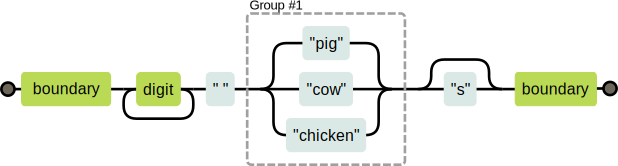
\includegraphics[width=10cm]{img/generated/re_pigchickens.pdf}
\vskip 1.5ex\index{traversal}

Our expression matches if we can find a path from the left side of the diagram to the right side. We keep a current position in the string, and every time we move through a box, we verify that the part of the string after our current position matches that box.

So if we try to match \lstinline`"the 3 pigs"` from position 4, our progress through the flow chart would look like this:

\begin{itemize}
\item 

At position 4, there is a word \index{boundary}boundary, so we can move past the first box.
\item 

Still at position 4, we find a digit, so we can also move past the second box.
\item 

At position 5, one path loops back to before the second (digit) box, while the other moves forward through the box that holds a single space character. There is a space here, not a digit, so we must take the second path.
\item 

We are now at position 6 (the start of \emph{pigs}) and at the three-way branch in the diagram. We don't see \emph{cow} or \emph{chicken} here, but we do see \emph{pig}, so we take that branch.
\item 

At position 9, after the three-way branch, one path skips the \emph{s} box and goes straight to the final word boundary, while the other path matches an \emph{s}. There is an \emph{s} character here, not a word boundary, so we go through the \emph{s} box.
\item 

We're at position 10 (the end of the string) and can match only a word \index{boundary}boundary. The end of a string counts as a word boundary, so we go through the last box and have successfully matched this string.
\end{itemize}

\label{regexp.backtracking}\section{Backtracking}\index{regular expression!backtracking}\index{binary number}\index{decimal number}\index{hexadecimal number}\index{flow diagram}\index{matching!algorithm}\index{backtracking}

The regular expression \lstinline`/\b([01]+b|[\da-f]+h|\d+)\b/` matches either a binary number followed by a \emph{b}, a hexadecimal number (that is, base 16, with the letters \emph{a} to \emph{f} standing for the digits 10 to 15) followed by an \emph{h}, or a regular decimal number with no suffix character. This is the corresponding diagram:

\vskip 1.5ex
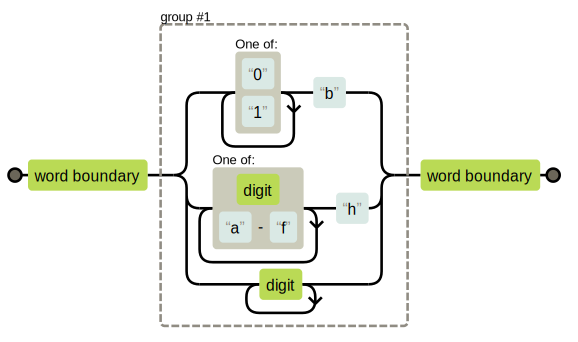
\includegraphics[width=10cm]{img/generated/re_number.pdf}
\vskip 1.5ex\index{branching}

When matching this expression, it will often happen that the top (binary) branch is entered even though the input does not actually contain a binary number. When matching the string \lstinline`"103"`, for example, it becomes clear only at the 3 that we are in the wrong branch. The string \emph{does} match the expression, just not the branch we are currently in.\index{backtracking}\index{search problem}

So the matcher \emph{backtracks}. When entering a branch, it remembers its current position (in this case, at the start of the string, just past the first boundary box in the diagram) so that it can go back and try another branch if the current one does not work out. For the string \lstinline`"103"`, after encountering the 3 character, it will start trying the branch for hexadecimal numbers, which fails again because there is no \emph{h} after the number. So it tries the decimal number branch. This one fits, and a match is reported after all.\index{matching!algorithm}

The matcher stops as soon as it finds a full match. This means that if multiple branches could potentially match a string, only the first one (ordered by where the branches appear in the regular expression) is used.

Backtracking also happens for \index{repetition}repetition operators like + and \lstinline`*`. If you match \lstinline`/^.*x/` against \lstinline`"abcxe"`, the \lstinline`.*` part will first try to consume the whole string. The engine will then realize that it needs an \emph{x} to match the pattern. Since there is no \emph{x} past the end of the string, the star operator tries to match one character less. But the matcher doesn't find an \emph{x} after \lstinline`abcx` either, so it backtracks again, matching the star operator to just \lstinline`abc`. \emph{Now} it finds an \emph{x} where it needs it and reports a successful match from positions 0 to 4.\index{performance}\index{complexity}

It is possible to write regular expressions that will do a \emph{lot} of backtracking. This problem occurs when a pattern can match a piece of input in many different ways. For example, if we get confused while writing a binary-number regular expression, we might accidentally write something like \lstinline`/([01]+)+b/`.

\vskip 1.5ex
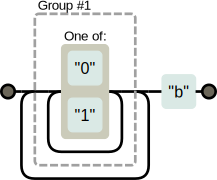
\includegraphics[width=6cm]{img/generated/re_slow.pdf}
\vskip 1.5ex\index{inner loop}\index{nesting!in regexps}

If that tries to match some long series of zeros and ones with no trailing \emph{b} character, the matcher first goes through the inner loop until it runs out of digits. Then it notices there is no \emph{b}, so it backtracks one position, goes through the outer loop once, and gives up again, trying to backtrack out of the inner loop once more. It will continue to try every possible route through these two loops. This means the amount of work \emph{doubles} with each additional character. For even just a few dozen characters, the resulting match will take practically forever.

\section{The replace method}\index{replace method}\index{regular expression}

String values have a \lstinline`replace` method that can be used to replace part of the string with another string.

\begin{lstlisting}
console.log("papa".replace("p", "m"));
// → mapa
\end{lstlisting}
\noindent\index{regular expression!flags}\index{regular expression!global}

The first argument can also be a regular expression, in which case the first match of the regular expression is replaced. When a \lstinline`g` option (for \emph{global}) is added to the regular expression, \emph{all} matches in the string will be replaced, not just the first.

\begin{lstlisting}
console.log("Borobudur".replace(/[ou]/, "a"));
// → Barobudur
console.log("Borobudur".replace(/[ou]/g, "a"));
// → Barabadar
\end{lstlisting}
\noindent\index{interface!design}\index{argument}

It would have been sensible if the choice between replacing one match or all matches was made through an additional argument to \lstinline`replace` or by providing a different method, \lstinline`replaceAll`. But for some unfortunate reason, the choice relies on a property of the regular expression instead.\index{grouping}\index{capture group}\index{dollar sign}\index{replace method}\index{regular expression!grouping}

The real power of using regular expressions with \lstinline`replace` comes from the fact that we can refer to matched groups in the replacement string. For example, say we have a big string containing the names of people, one name per line, in the format \lstinline`Lastname, Firstname`. If we want to swap these names and remove the comma to get a \lstinline`Firstname Lastname` format, we can use the following code:

\begin{lstlisting}
console.log(
  "Liskov, Barbara\nMcCarthy, John\nWadler, Philip"
    .replace(/(\w+), (\w+)/g, "$2 $1"));
// → Barbara Liskov
//   John McCarthy
//   Philip Wadler
\end{lstlisting}
\noindent

The \lstinline`$1` and \lstinline`$2` in the replacement string refer to the parenthesized groups in the pattern. \lstinline`$1` is replaced by the text that matched against the first group, \lstinline`$2` by the second, and so on, up to \lstinline`$9`. The whole match can be referred to with \lstinline`$&`.\index{function!higher-order}\index{grouping}\index{capture group}

It is possible to pass a function—rather than a string—as the second argument to \lstinline`replace`. For each replacement, the function will be called with the matched groups (as well as the whole match) as arguments, and its return value will be inserted into the new string.

Here's a small example:

\begin{lstlisting}
let s = "the cia and fbi";
console.log(s.replace(/\b(fbi|cia)\b/g,
            str => str.toUpperCase()));
// → the CIA and FBI
\end{lstlisting}
\noindent

Here's a more interesting one:

\begin{lstlisting}
let stock = "1 lemon, 2 cabbages, and 101 eggs";
function minusOne(match, amount, unit) {
  amount = Number(amount) - 1;
  if (amount == 1) { // only one left, remove the 's'
    unit = unit.slice(0, unit.length - 1);
  } else if (amount == 0) {
    amount = "no";
  }
  return amount + " " + unit;
}
console.log(stock.replace(/(\d+) (\w+)/g, minusOne));
// → no lemon, 1 cabbage, and 100 eggs
\end{lstlisting}
\noindent

This takes a string, finds all occurrences of a number followed by an alphanumeric word, and returns a string wherein every such occurrence is decremented by one.

The \lstinline`(\d+)` group ends up as the \lstinline`amount` argument to the function, and the \lstinline`(\w+)` group gets bound to \lstinline`unit`. The function converts \lstinline`amount` to a number—which always works since it matched \lstinline`\d+`—and makes some adjustments in case there is only one or zero left.

\section{Greed}\index{greed}\index{regular expression}

It is possible to use \lstinline`replace` to write a function that removes all \index{comment}comments from a piece of JavaScript \index{code}code. Here is a first attempt:

\begin{lstlisting}
function stripComments(code) {
  return code.replace(/\/\/.*|\/\*[^]*\*\//g, "");
}
console.log(stripComments("1 + /* 2 */3"));
// → 1 + 3
console.log(stripComments("x = 10;// ten!"));
// → x = 10;
console.log(stripComments("1 /* a */+/* b */ 1"));
// → 1  1
\end{lstlisting}
\noindent\index{period character}\index{slash character}\index{newline character}\index{empty set}\index{block comment}\index{line comment}

The part before the \emph{or} operator matches two slash characters followed by any number of non-newline characters. The part for multiline comments is more involved. We use \lstinline`[^]` (any character that is not in the empty set of characters) as a way to match any character. We cannot just use a period here because block comments can continue on a new line, and the period character does not match newline characters.

But the output for the last line appears to have gone wrong. Why?\index{backtracking}\index{greed}\index{regular expression}

The \lstinline`[^]*` part of the expression, as I described in the section on backtracking, will first match as much as it can. If that causes the next part of the pattern to fail, the matcher moves back one character and tries again from there. In the example, the matcher first tries to match the whole rest of the string and then moves back from there. It will find an occurrence of \lstinline`*/` after going back four characters and match that. This is not what we wanted—the intention was to match a single comment, not to go all the way to the end of the code and find the end of the last block comment.

Because of this behavior, we say the repetition operators (\lstinline`+`, \lstinline`*`, \lstinline`?`, and \lstinline`{}`) are \emph{\index{greed}greedy}, meaning they match as much as they can and backtrack from there. If you put a \index{question mark}question mark after them (\lstinline`+?`, \lstinline`*?`, \lstinline`??`, \lstinline`{}?`), they become nongreedy and start by matching as little as possible, matching more only when the remaining pattern does not fit the smaller match.

And that is exactly what we want in this case. By having the star match the smallest stretch of characters that brings us to a \lstinline`*/`, we consume one block comment and nothing more.

\begin{lstlisting}
function stripComments(code) {
  return code.replace(/\/\/.*|\/\*[^]*?\*\//g, "");
}
console.log(stripComments("1 /* a */+/* b */ 1"));
// → 1 + 1
\end{lstlisting}
\noindent

A lot of \index{bug}bugs in \index{regular expression}regular expression programs can be traced to unintentionally using a greedy operator where a nongreedy one would work better. When using a \index{repetition}repetition operator, consider the nongreedy variant first.

\section{Dynamically creating RegExp objects}\index{regular expression!creation}\index{underscore character}\index{RegExp class}

There are cases where you might not know the exact \index{pattern}pattern you need to match against when you are writing your code. Say you want to look for the user's name in a piece of text and enclose it in underscore characters to make it stand out. Since you will know the name only once the program is actually running, you can't use the slash-based notation.

But you can build up a string and use the \lstinline`RegExp` \index{constructor}constructor on that. Here's an example:

\begin{lstlisting}
let name = "harry";
let text = "Harry is a suspicious character.";
let regexp = new RegExp("\\b(" + name + ")\\b", "gi");
console.log(text.replace(regexp, "_$1_"));
// → _Harry_ is a suspicious character.
\end{lstlisting}
\noindent\index{regular expression!flags}\index{backslash character!in regular expressions}

When creating the \lstinline`\b` \index{boundary}boundary markers, we have to use two backslashes because we are writing them in a normal string, not a slash-enclosed regular expression. The second argument to the \lstinline`RegExp` constructor contains the options for the regular expression—in this case, \lstinline`"gi"` for global and case insensitive.

But what if the name is \lstinline`"dea+hl[]rd"` because our user is a \index{nerd}nerdy teenager? That would result in a nonsensical regular expression that won't actually match the user's name.\index{backslash character!in regular expressions}\index{escaping!in regexps}\index{regular expression!escaping}

To work around this, we can add backslashes before any character that has a special meaning.

\begin{lstlisting}
let name = "dea+hl[]rd";
let text = "This dea+hl[]rd guy is super annoying.";
let escaped = name.replace(/[\\[.+*?(){|^$]/g, "\\$&");
let regexp = new RegExp("\\b" + escaped + "\\b", "gi");
console.log(text.replace(regexp, "_$&_"));
// → This _dea+hl[]rd_ guy is super annoying.
\end{lstlisting}
\noindent

\section{The search method}\index{regular expression!methods}\index{indexOf method}\index{search method}

The \lstinline`indexOf` method on strings cannot be called with a regular expression. But there is another method, \lstinline`search`, that does expect a regular expression. Like \lstinline`indexOf`, it returns the first index on which the expression was found, or -1 when it wasn't found.

\begin{lstlisting}
console.log("  word".search(/\S/));
// → 2
console.log("    ".search(/\S/));
// → -1
\end{lstlisting}
\noindent

Unfortunately, there is no way to indicate that the match should start at a given offset (like we can with the second argument to \lstinline`indexOf`), which would often be useful.

\section{The lastIndex property}\index{exec method}\index{regular expression}

The \lstinline`exec` method similarly does not provide a convenient way to start searching from a given position in the string. But it does provide an \emph{in}convenient way.\index{regular expression!matching}\index{matching}\index{source property}\index{lastIndex property}

Regular expression objects have properties. One such property is \lstinline`source`, which contains the string that expression was created from. Another property is \lstinline`lastIndex`, which controls, in some limited circumstances, where the next match will start.\index{interface!design}\index{exec method}\index{regular expression!global}

Those circumstances are that the regular expression must have the global (\lstinline`g`) or sticky (\lstinline`y`) option enabled, and the match must happen through the \lstinline`exec` method. Again, a less confusing solution would have been to just allow an extra argument to be passed to \lstinline`exec`, but confusion is an essential feature of JavaScript's regular expression interface.

\begin{lstlisting}
let pattern = /y/g;
pattern.lastIndex = 3;
let match = pattern.exec("xyzzy");
console.log(match.index);
// → 4
console.log(pattern.lastIndex);
// → 5
\end{lstlisting}
\noindent\index{side effect}\index{lastIndex property}

If the match was successful, the call to \lstinline`exec` automatically updates the \lstinline`lastIndex` property to point after the match. If no match was found, \lstinline`lastIndex` is set back to zero, which is also the value it has in a newly constructed regular expression object.

The difference between the global and the sticky options is that, when sticky is enabled, the match will succeed only if it starts directly at \lstinline`lastIndex`, whereas with global, it will search ahead for a position where a match can start.

\begin{lstlisting}
let global = /abc/g;
console.log(global.exec("xyz abc"));
// → ["abc"]
let sticky = /abc/y;
console.log(sticky.exec("xyz abc"));
// → null
\end{lstlisting}
\noindent\index{bug}

When using a shared regular expression value for multiple \lstinline`exec` calls, these automatic updates to the \lstinline`lastIndex` property can cause problems. Your regular expression might be accidentally starting at an index that was left over from a previous call.

\begin{lstlisting}
let digit = /\d/g;
console.log(digit.exec("here it is: 1"));
// → ["1"]
console.log(digit.exec("and now: 1"));
// → null
\end{lstlisting}
\noindent\index{regular expression!global}\index{match method}

Another interesting effect of the global option is that it changes the way the \lstinline`match` method on strings works. When called with a global expression, instead of returning an array similar to that returned by \lstinline`exec`, \lstinline`match` will find \emph{all} matches of the pattern in the string and return an array containing the matched strings.

\begin{lstlisting}
console.log("Banana".match(/an/g));
// → ["an", "an"]
\end{lstlisting}
\noindent

So be cautious with global regular expressions. The cases where they are necessary—calls to \lstinline`replace` and places where you want to explicitly use \lstinline`lastIndex`—are typically the only places where you want to use them.

\subsection{Looping over matches}\index{lastIndex property}\index{exec method}\index{loop}

A common thing to do is to scan through all occurrences of a pattern in a string, in a way that gives us access to the match object in the loop body. We can do this by using \lstinline`lastIndex` and \lstinline`exec`.

\begin{lstlisting}
let input = "A string with 3 numbers in it... 42 and 88.";
let number = /\b\d+\b/g;
let match;
while (match = number.exec(input)) {
  console.log("Found", match[0], "at", match.index);
}
// → Found 3 at 14
//   Found 42 at 33
//   Found 88 at 40
\end{lstlisting}
\noindent\index{while loop}\index{= operator!as expression}\index{binding!as state}

This makes use of the fact that the value of an \index{assignment}assignment expression (\lstinline`=`) is the assigned value. So by using \lstinline`match = number.exec(input)` as the condition in the \lstinline`while` statement, we perform the match at the start of each iteration, save its result in a binding, and stop looping when no more matches are found.

\label{regexp.ini}\section{Parsing an INI file}\index{comment}\index{file format}\index{enemies example}\index{INI file}

To conclude the chapter, we'll look at a problem that calls for \index{regular expression}regular expressions. Imagine we are writing a program to automatically collect information about our enemies from the \index{Internet}Internet. (We will not actually write that program here, just the part that reads the \index{configuration}configuration file. Sorry.) The configuration file looks like this:

\begin{lstlisting}
searchengine=https://duckduckgo.com/?q=$1
spitefulness=9.7

; comments are preceded by a semicolon...
; each section concerns an individual enemy
[larry]
fullname=Larry Doe
type=kindergarten bully
website=http://www.geocities.com/CapeCanaveral/11451

[davaeorn]
fullname=Davaeorn
type=evil wizard
outputdir=/home/marijn/enemies/davaeorn
\end{lstlisting}
\noindent\index{grammar}

The exact rules for this format (which is a widely used format, usually called an \emph{INI} file) are as follows:

\begin{itemize}
\item 

Blank lines and lines starting with semicolons are ignored.
\item 

Lines wrapped in \lstinline`[` and \lstinline`]` start a new \index{section}section.
\item 

Lines containing an alphanumeric identifier followed by an \lstinline`=` character add a setting to the current section.
\item 

Anything else is invalid.
\end{itemize}

Our task is to convert a string like this into an object whose properties hold strings for settings written before the first section header and subobjects for sections, with those subobjects holding the section's settings.\index{carriage return}\index{line break}\index{newline character}

Since the format has to be processed \index{line}line by line, splitting up the file into separate lines is a good start. We saw the \lstinline`split` method in \hyperref[data.split]{Chapter 4}. Some operating systems, however, use not just a newline character to separate lines but a carriage return character followed by a newline (\lstinline`"\r\n"`). Given that the \lstinline`split` method also allows a regular expression as its argument, we can use a regular expression like \lstinline`/\r?\n/` to split in a way that allows both \lstinline`"\n"` and \lstinline`"\r\n"` between lines.

\begin{lstlisting}
function parseINI(string) {
  // Start with an object to hold the top-level fields
  let result = {};
  let section = result;
  string.split(/\r?\n/).forEach(line => {
    let match;
    if (match = line.match(/^(\w+)=(.*)$/)) {
      section[match[1]] = match[2];
    } else if (match = line.match(/^\[(.*)\]$/)) {
      section = result[match[1]] = {};
    } else if (!/^\s*(;.*)?$/.test(line)) {
      throw new Error("Line '" + line + "' is not valid.");
    }
  });
  return result;
}

console.log(parseINI(`
name=Vasilis
[address]
city=Tessaloniki`));
// → {name: "Vasilis", address: {city: "Tessaloniki"}}
\end{lstlisting}
\noindent\index{parseINI function}\index{parsing}

The code goes over the file's lines and builds up an object. Properties at the top are stored directly into that object, whereas properties found in sections are stored in a separate section object. The \lstinline`section` binding points at the object for the current section.

There are two kinds of significant lines—section headers or property lines. When a line is a regular property, it is stored in the current section. When it is a section header, a new section object is created, and \lstinline`section` is set to point at it.\index{caret character}\index{dollar sign}\index{boundary}

Note the recurring use of \lstinline`^` and \lstinline`$` to make sure the expression matches the whole line, not just part of it. Leaving these out results in code that mostly works but behaves strangely for some input, which can be a difficult bug to track down.\index{if keyword}\index{assignment}\index{= operator!as expression}

The pattern \lstinline`if (match = string.match(...))` is similar to the trick of using an assignment as the condition for \lstinline`while`. You often aren't sure that your call to \lstinline`match` will succeed, so you can access the resulting object only inside an \lstinline`if` statement that tests for this. To not break the pleasant chain of \lstinline`else if` forms, we assign the result of the match to a binding and immediately use that assignment as the test for the \lstinline`if` statement.\index{parentheses!in regular expressions}

If a line is not a section header or a property, the function checks whether it is a comment or an empty line using the expression \lstinline`/^\s*(;.*)?$/`. Do you see how it works? The part between the parentheses will match comments, and the \lstinline`?` makes sure it also matches lines containing only whitespace. When a line doesn't match any of the expected forms, the function throws an exception.

\section{International characters}\index{internationalization}\index{Unicode}\index{regular expression!internationalization}

Because of JavaScript's initial simplistic implementation and the fact that this simplistic approach was later set in stone as \index{standard}standard behavior, JavaScript's regular expressions are rather dumb about characters that do not appear in the English language. For example, as far as JavaScript's regular expressions are concerned, a ``\index{word
character}word
character'' is only one of the 26 characters in the Latin alphabet (uppercase or lowercase), decimal digits, and, for some reason, the underscore character. Things like \emph{é} or \emph{β}, which most definitely are word characters, will not match \lstinline`\w` (and \emph{will} match uppercase \lstinline`\W`, the nonword category).\index{whitespace!matching}

By a strange historical accident, \lstinline`\s` (whitespace) does not have this problem and matches all characters that the Unicode standard considers whitespace, including things like the \index{nonbreaking space}nonbreaking space and the \index{Mongolian vowel separator}Mongolian vowel separator.

Another problem is that, by default, regular expressions work on code units, as discussed in \hyperref[higher_order.code_units]{Chapter 5}, not actual characters. This means characters that are composed of two code units behave strangely.

\begin{lstlisting}
console.log(/$<🍎>${3}/.test("$<🍎🍎🍎>$"));
// → false
console.log(/<.>/.test("<$<🌹>$>"));
// → false
console.log(/<.>/u.test("<$<🌹>$>"));
// → true
\end{lstlisting}
\noindent

The problem is that the 🍎 in the first line is treated as two code units, and the \lstinline`{3}` part is applied only to the second one. Similarly, the dot matches a single code unit, not the two that make up the rose \index{emoji}emoji.

You must add a \lstinline`u` option (for \index{Unicode}Unicode) to your regular expression to make it treat such characters properly. The wrong behavior remains the default, unfortunately, because changing that might cause problems for existing code that depends on it.\index{character category}\index{Unicode!property}

Though this was only just standardized and is, at the time of writing, not widely supported yet, it is possible to use \lstinline`\p` in a regular expression (that must have the Unicode option enabled) to match all characters to which the Unicode standard assigns a given property.

\begin{lstlisting}
console.log(/\p{Script=Greek}/u.test("α"));
// → true
console.log(/\p{Script=Arabic}/u.test("α"));
// → false
console.log(/\p{Alphabetic}/u.test("α"));
// → true
console.log(/\p{Alphabetic}/u.test("!"));
// → false
\end{lstlisting}
\noindent

Unicode defines a number of useful properties, though finding the one that you need may not always be trivial. You can use the \lstinline`\p{Property=Value}` notation to match any character that has the given value for that property. If the property name is left off, as in \lstinline`\p{Name}`, the name is assumed to be either a binary property such as \lstinline`Alphabetic` or a category such as \lstinline`Number`.

\label{regexp.summary_regexp}\section{Summary}

Regular expressions are objects that represent patterns in strings. They use their own language to express these patterns.

\noindent\begin{tabular}{ll}
\lstinline`/abc/` &
A sequence of characters
\tabularnewline
\lstinline`/[abc]/` &
Any character from a set of characters
\tabularnewline
\lstinline`/[^abc]/` &
Any character \emph{not} in a set of characters
\tabularnewline
\lstinline`/[0-9]/` &
Any character in a range of characters
\tabularnewline
\lstinline`/x+/` &
One or more occurrences of the pattern \lstinline`x`
\tabularnewline
\lstinline`/x+?/` &
One or more occurrences, nongreedy
\tabularnewline
\lstinline`/x*/` &
Zero or more occurrences
\tabularnewline
\lstinline`/x?/` &
Zero or one occurrence
\tabularnewline
\lstinline`/x{2,4}/` &
Two to four occurrences
\tabularnewline
\lstinline`/(abc)/` &
A group
\tabularnewline
\lstinline`/a|b|c/` &
Any one of several patterns
\tabularnewline
\lstinline`/\d/` &
Any digit character
\tabularnewline
\lstinline`/\w/` &
An alphanumeric character (``word character'')
\tabularnewline
\lstinline`/\s/` &
Any whitespace character
\tabularnewline
\lstinline`/./` &
Any character except newlines
\tabularnewline
\lstinline`/\b/` &
A word boundary
\tabularnewline
\lstinline`/^/` &
Start of input
\tabularnewline
\lstinline`/$/` &
End of input
\tabularnewline
\end{tabular}

A regular expression has a method \lstinline`test` to test whether a given string matches it. It also has a method \lstinline`exec` that, when a match is found, returns an array containing all matched groups. Such an array has an \lstinline`index` property that indicates where the match started.

Strings have a \lstinline`match` method to match them against a regular expression and a \lstinline`search` method to search for one, returning only the starting position of the match. Their \lstinline`replace` method can replace matches of a pattern with a replacement string or function.

Regular expressions can have options, which are written after the closing slash. The \lstinline`i` option makes the match case insensitive. The \lstinline`g` option makes the expression \emph{global}, which, among other things, causes the \lstinline`replace` method to replace all instances instead of just the first. The \lstinline`y` option makes it sticky, which means that it will not search ahead and skip part of the string when looking for a match. The \lstinline`u` option turns on Unicode mode, which fixes a number of problems around the handling of characters that take up two code units.

Regular expressions are a sharp \index{tool}tool with an awkward handle. They simplify some tasks tremendously but can quickly become unmanageable when applied to complex problems. Part of knowing how to use them is resisting the urge to try to shoehorn things that they cannot cleanly express into them.

\section{Exercises}\index{debugging}\index{bug}

It is almost unavoidable that, in the course of working on these exercises, you will get confused and frustrated by some regular expression's inexplicable \index{behavior}behavior. Sometimes it helps to enter your expression into an online tool like \href{https://www.debuggex.com/}{\emph{https://debuggex.com}} to see whether its visualization corresponds to what you intended and to \index{experiment}experiment with the way it responds to various input strings.

\subsection{Regexp golf}\index{program size}\index{code golf}\index{regexp golf (exercise)}

\emph{Code golf} is a term used for the game of trying to express a particular program in as few characters as possible. Similarly, \emph{regexp golf} is the practice of writing as tiny a regular expression as possible to match a given pattern, and \emph{only} that pattern.\index{boundary}\index{matching}

For each of the following items, write a \index{regular expression}regular expression to test whether any of the given substrings occur in a string. The regular expression should match only strings containing one of the substrings described. Do not worry about word boundaries unless explicitly mentioned. When your expression works, see whether you can make it any smaller.

\begin{enumerate}
\item 

\emph{car} and \emph{cat}
\item 

\emph{pop} and \emph{prop}
\item 

\emph{ferret}, \emph{ferry}, and \emph{ferrari}
\item 

Any word ending in \emph{ious}
\item 

A whitespace character followed by a period, comma, colon, or semicolon
\item 

A word longer than six letters
\item 

A word without the letter \emph{e} (or \emph{E})
\end{enumerate}

Refer to the table in the \hyperref[regexp.summary_regexp]{chapter summary} for help. Test each solution with a few test strings.

\subsection{Quoting style}\index{quoting style (exercise)}\index{single-quote character}\index{double-quote character}

Imagine you have written a story and used single \index{quotation mark}quotation marks throughout to mark pieces of dialogue. Now you want to replace all the dialogue quotes with double quotes, while keeping the single quotes used in contractions like \emph{aren't}.\index{replace method}

Think of a pattern that distinguishes these two kinds of quote usage and craft a call to the \lstinline`replace` method that does the proper replacement.

\subsection{Numbers again}\index{sign}\index{fractional number}\index{syntax!number}\index{minus}\index{plus character}\index{exponent}\index{scientific notation}\index{period character}

Write an expression that matches only JavaScript-style \index{number}numbers. It must support an optional minus \emph{or} plus sign in front of the number, the decimal dot, and exponent notation—\lstinline`5e-3` or \lstinline`1E10`—again with an optional sign in front of the exponent. Also note that it is not necessary for there to be digits in front of or after the dot, but the number cannot be a dot alone. That is, \lstinline`.5` and \lstinline`5.` are valid JavaScript numbers, but a lone dot \emph{isn't}.
